\documentclass[11pt]{article}

\usepackage{fontspec}
\usepackage{amsmath}
\usepackage{polyglossia}
\setmainlanguage{turkish}
\usepackage{geometry}
\geometry{a4paper, margin=2.5cm}
\usepackage{graphicx}
\usepackage{booktabs}
\usepackage{float}
\usepackage{xcolor}
\usepackage{hyperref}
\hypersetup{colorlinks=true, linkcolor=blue, urlcolor=blue}

\graphicspath{{figures/}}

\title{\textbf{YKS ``Sallamasyon'' III:\\
Sıfırdan Tahmin --- Hiçbir Cevap Bilinmeden Cevap Anahtarı Kestirimi}}
\author{Hamza Yiğit Kültür \quad\textbullet\quad İsmail Güler\\[2pt]
\small \texttt{sallamasyon-yks} --- NVIDIA GH200 (Grace 72-core + H100)}
\date{\today}

\begin{document}
\maketitle

\begin{abstract}
\noindent
Önceki raporlar, bazı cevapların bilindiği ``boşluk doldurma'' senaryosuna
odaklanmıştı. Bu üçüncü rapor ise en zor ve en saf duruma adanmıştır:
\textbf{sıfırdan tahmin} ($k=0$), yani hiçbir cevap bilinmeden bir sınav
testinin tüm cevap anahtarının baştan kestirilmesi. Tüm modeller yalnızca
2018--2024'te eğitilir; 2025 dokunulmamış test setidir. Sonuçlar nettir ve
büyük ölçüde olumsuzdur: şık dağılımı düzgüne çok yakın ve ders bazlı ``en sık
şık'' yıllar arasında \emph{kararsız} olduğundan (6 dersten yalnızca 1'inde
train ile 2025 örtüşür), frekans ve pozisyon temelli yaklaşımlar neredeyse
işe yaramaz. Sıfırdan tahminde tek anlamlı strateji, \emph{dengeli ve ardarda
tekrarsız bir dizi üretmektir}: train'de seçilen bir A--E permutasyon döngüsü
($\textsc{PermCycle}$) $\%23.37$ ile rastgeleyi ($\%20.03$) en çok geçen
modeldir ve ulaşılabilir tavanın ($\%25.09$, oracle) çok yakınındadır. Boşluk
doldurmada güçlü olan dengeleme ve derin GRU, sıfırdan tahminde rastgelenin
\emph{altına} düşer.
\end{abstract}

\section{Sıfırdan Tahmin Nedir, Neden Zordur?}
``Sallamasyon''un en uç biçimi, elde hiçbir doğru cevap olmadan tüm testi
kestirmektir. Boşluk doldurmadan (önceki rapor) temel farkı: orada bilinen
komşu cevaplar hem dengeleme bütçesini hem yerel tekrar kısıtını
\emph{çapalardı}. Sıfırdan tahminde böyle bir çapa yoktur; model yalnızca
geçmiş yılların \emph{global} yapısına yaslanabilir. Bu yapı zayıfsa---ki bu
çalışmada öyledir---tavan da düşüktür.

\section{Veri ve Sızıntı Güvencesi}
Veri, önceki raporlarla aynı yapılandırılmış cevap anahtarıdır: eğitim
\textbf{2018--2024} ($2034$ cevap, $56$ test dizisi), bağımsız değerlendirme
\textbf{2025} ($291$ cevap, $8$ test dizisi). Tüm modeller ve seçilen
parametreler (permutasyon, frekans tabloları) yalnızca eğitimden türetilir;
2025 yalnızca ölçüm için kullanılır (\texttt{check\_leakage.py} ile
doğrulanmıştır). Tek istisna, açıkça etiketlenen \emph{oracle} üst sınırıdır:
o, 2025'e bakarak en iyi permutasyonu seçer ve bir model değil, ``ulaşılabilir
tavan'' referansıdır.

\section{Neden Frekans ve Pozisyon İşe Yaramaz?}
Birinci raporda şık dağılımının düzgüne çok yakın olduğunu ($\chi^2=3.35$,
anlamsız) göstermiştik. Sıfırdan tahmin için asıl öldürücü bulgu, ders bazlı
``en sık şık''ın \emph{yıllar arasında kararsız} olmasıdır
(Şekil~\ref{fig:freq}): eğitimdeki en sık şık ile 2025'teki en sık şık
\textbf{6 dersten yalnızca 1'inde} aynıdır. Bu yüzden ``bu derste genelde X
çıkar'' kuralı 2025'e taşınamaz; frekans temelli \textsc{GlobalFreq} yalnızca
$\%21.99$, pozisyonel argmax ise rastgelenin \emph{altında} ($\%18.56$) kalır.

\begin{figure}[H]
\centering
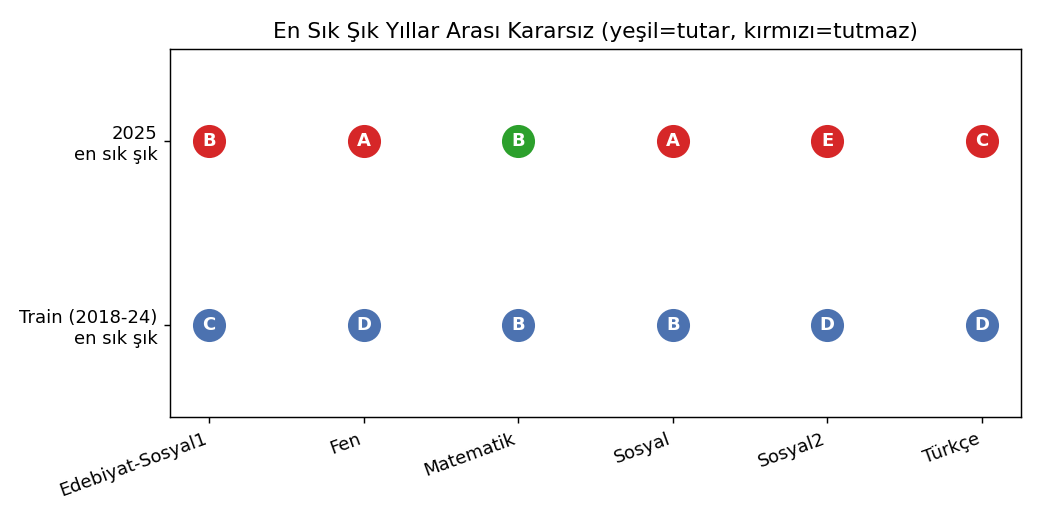
\includegraphics[width=0.85\textwidth]{coldstart_frekans_kararsiz.png}
\caption{Ders bazlı ``en sık şık''ın yıllar arası kararsızlığı. Üst satır
2025, alt satır eğitim. Yeşil yalnızca tek derste (tutar); kalan beşinde
eğitimden öğrenilen en sık şık 2025'te değişir (kırmızı).}
\label{fig:freq}
\end{figure}

\section{Değerlendirme Protokolü}
\textbf{Doğruluk tanımı.} Doğruluk, 2025 test setinde doğru tahmin edilen
soru sayısının toplam soru sayısına oranıdır (yüzde); rastgele beklenti
$\%20$'dir. Sıfırdan tahminde ($k=0$) tüm pozisyonlar gizli olduğundan, oran
testin tamamı üzerinden hesaplanır.

\textbf{Tur sayısı.} Rastgelelik içeren modeller (Rastgele, BalancedShuffle)
\textbf{$1500$ bağımsız tur} ile değerlendirilip \emph{ortalama $\pm$ standart
sapma} raporlanır. Deterministik modeller (PermCycle, GlobalFreq, Markov,
Dengeleme, Pozisyonel ve eğitilmiş derin modeller) sıfırdan tahminde sabit
çıktı verdiğinden tek değerle ($\pm 0$) raporlanır.

\section{Modeller}
Tüm modeller sıfırdan tahmin ($k=0$) modunda, aynı test dizilerinde
değerlendirildi.

\paragraph{Mevcut modeller.} \emph{Rastgele} (referans), \emph{GlobalFreq}
(ders bazlı en sık şık), \emph{Markov} (sıfırdan tahminde komşu olmadığı için
yalnızca öncül dağılıma düşer), \emph{Dengeleme} (boşluk doldurma aracı),
\emph{GRU} ve \emph{MaskedBERT} (derin, GH200; MLM ile eğitilmiş).

\paragraph{Yeni sıfırdan-tahmin modelleri.}
\begin{itemize}
  \item \textbf{PermCycle.} Dengeli ve ardarda tekrarsız bir dizi üretici.
  Train'de en yüksek isabeti veren A--E permutasyon \emph{döngüsünü} seçer
  (eğitimde $BAECD$) ve diziye sıra ile uygular. Her $5$'lik blokta tüm şıklar
  bir kez geçtiğinden hem dengeleme hem tekrar-kaçınma kısıtını otomatik
  sağlar. Permutasyon seçimi yalnızca eğitim isabetine dayanır (sızıntısız).
  \item \textbf{BalancedShuffle.} Hedef orana göre dengeli ama deterministik
  olmayan, ardarda tekrarı bozan karıştırıcı. PermCycle'ın esnek/rastgele hali.
  \item \textbf{Pozisyonel.} $P(\text{şık}\mid\text{ders},\text{soru\_no})$
  argmax; pozisyonel örüntü testi (negatif kontrol).
\end{itemize}

\section{Sonuçlar}
\begin{table}[H]
\centering
\caption{Sıfırdan tahmin ($k=0$) doğrulukları, 2025 test seti. Kazanç:
rastgeleye karşı puan farkı; kırmızı negatif. Kalın: en iyi.}
\label{tab:cold}
\begin{tabular}{lcc}
\toprule
Model & 2025 Doğruluk (\%) & Kazanç (puan) \\
\midrule
\textbf{PermCycle} & \textbf{23.37} & +3.36 \\
GlobalFreq & 21.99 & +1.99 \\
MaskedBERT & 21.65 & +1.64 \\
Markov & 21.31 & +1.30 \\
BalancedShuffle & 20.04$\pm$2.4 & +0.04 \\
Rastgele & 20.01$\pm$2.3 & +0.00 \\
Pozisyonel & 18.56 & \textcolor{red}{-1.45} \\
GRU & 17.18 & \textcolor{red}{-2.82} \\
Dengeleme & 15.12 & \textcolor{red}{-4.89}

\\
\bottomrule
\end{tabular}
\end{table}

\begin{figure}[H]
\centering
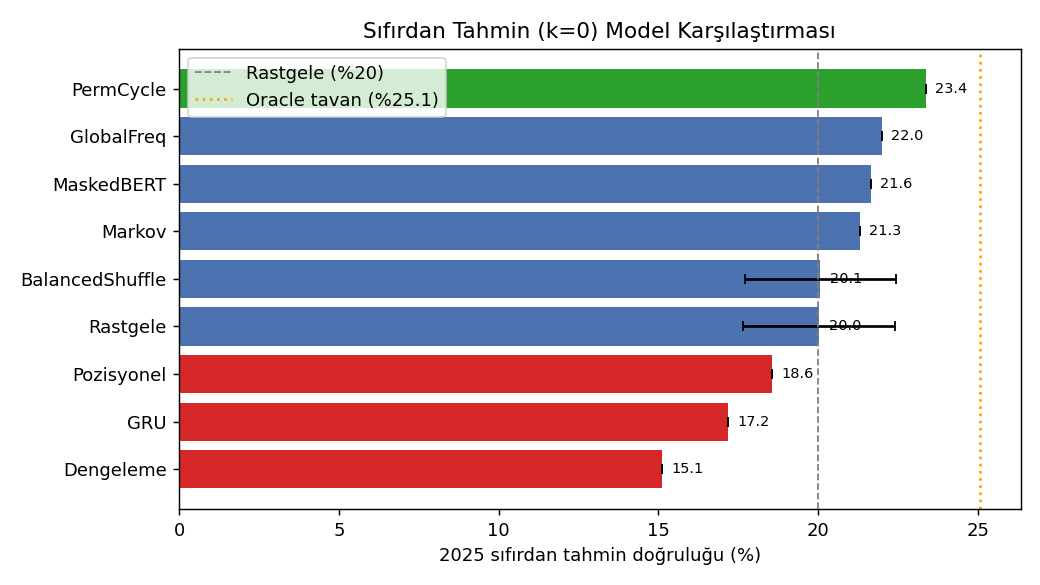
\includegraphics[width=0.92\textwidth]{coldstart_karsilastirma.png}
\caption{Sıfırdan tahmin model karşılaştırması. Yeşil: en iyi
($\textsc{PermCycle}$); kırmızı: rastgelenin altına düşen ``çöken'' modeller.
Gri kesikli rastgele ($\%20$), turuncu noktalı oracle tavanını ($\%25.1$)
gösterir.}
\label{fig:cmp}
\end{figure}

\section{Derin Analiz: Hangi Model Neden Böyle Davranır?}
\begin{itemize}
  \item \textbf{PermCycle ($\%23.37$, +3.34) --- tavanın yakınında.} Sıfırdan
  tahminde sömürülebilecek tek yapı, ÖSYM'nin dengeli ve ardarda tekrarsız
  cevap dizmesidir. PermCycle bu iki kısıtı doğrudan inşa eder. Oracle
  tavanı $\%25.09$ olduğundan, train'den seçilen döngü tavanın yalnızca
  $\sim 1.7$ puan altındadır---yani bu yaklaşım neredeyse en iyisini yapar.
  \item \textbf{Dengeleme ($\%15.12$, $-4.91$) --- çöker.} Bilinen cevap
  olmadan dengeleme, ilk tahmini atıp sonra o şıkkı baskılayarak gerçekle
  hizalanmayan deterministik bir döngü üretir. Boşluk doldurmanın yıldızı,
  sıfırdan tahminin en kötüsüdür.
  \item \textbf{GRU ($\%17.18$, $-2.85$) --- çöker.} Maskeli-dil-modeli ile
  eğitilen GRU, çevresinde bağlam (bilinen komşu) \emph{beklemeye} koşullanır.
  Sıfırdan tahminde hiç bağlam olmadığından kararsız, rastgele-altı çıktı
  üretir. (Not: aynı GRU, bilinen oran yüksekken çok daha iyidir.)
  \item \textbf{Pozisyonel ($\%18.56$, $-1.47$) --- işe yaramaz.} ``$k$.\ soru
  genelde X'tir'' diye bir kural olmadığından rastgelenin altına düşer.
  \item \textbf{Frekans/derin modeller ($\sim\%22$) --- marjinal.}
  \textsc{GlobalFreq} ve \textsc{MaskedBERT} rastgeleyi $\sim 2$ puan geçer;
  ikisi de örtük olarak ``dengeli, hafif eğimli'' bir dağılım üretir ama
  yıllar-arası kararsızlık nedeniyle PermCycle'ı yakalayamaz.
\end{itemize}

\section{Sonuç}
Sıfırdan tahmin, YKS cevap anahtarları için neredeyse bir taş duvardır: şık
dağılımı düzgüne yakın ve yıllar arası kararsız olduğundan, hiçbir cevap
bilinmeden ulaşılabilecek tavan $\sim\%25$, pratikte sızıntısız en iyi model
$\%23.37$'dir. Tek işe yarayan içgörü, ÖSYM'nin \emph{dengeli ve ardarda
tekrarsız} dizmesidir; bunu doğrudan inşa eden basit bir permutasyon döngüsü,
GH200 üzerinde eğitilen derin modelleri dahi geçer. Pratik çıkarım: hiçbir
soruyu bilmeden ``sallayan'' biri için en akıllıca strateji, kâğıda
\emph{dengeli ve hiç ardarda tekrar etmeyen} bir şık dizisi yazmaktır---ama
beklenen kazanç rastgeleye göre yalnızca birkaç puandır. Asıl kazanç, önceki
raporda gösterildiği gibi, \emph{en az birkaç cevabın bilindiği} durumlardan
gelir.

\paragraph{Tekrarlanabilirlik.} İşlem hattı: \texttt{check\_leakage.py}
$\rightarrow$ \texttt{eval\_coldstart.py} $\rightarrow$
\texttt{analyze\_coldstart.py} $\rightarrow$ \texttt{build\_report3.py}.

\end{document}
